\documentclass[parskip=full]{scrartcl}
\usepackage[utf8]{inputenc} % use utf8 file encoding for TeX sources
\usepackage[T1]{fontenc}    % avoid garbled Unicode text in pdf
\usepackage[german]{babel}  % german hyphenation, quotes, etc
\usepackage{hyperref}       % detailed hyperlink/pdf configuration
\hypersetup{                % ‘texdoc hyperref‘ for options
	pdftitle={Entwurf},%
	bookmarks=true,%
}
\usepackage{graphicx}       % provides commands for including figures
\usepackage{csquotes}       % provides \enquote{} macro for "quotes"
\usepackage{scrpage2}
\pagestyle{scrheadings}
\usepackage{float}

%\clearscrheadfoot
\ohead{BPTI: Gruppe 03=\{Niklas Metz, Felix Bachmann\}, Aufgabenblatt 1, WS 2017/18}

\begin{document}
	\setcounter{section}{1}
	\section*{Aufgabe 1: Hardwarebeschreibungssprachen}
		\subsection{ABEL}
			ABEL steht für Advanced Boolean Equation Language und wurde hauptsächlich in den 80ern und 90ern für einfache logische Schaltungen, also vorallem kleine FPGAs, verwendet. ABEL unterstützt eine breite Anzahl an Eingabemethoden von High-Level Gleichungen bis zu einfach Wahrheitstabellen. 
			Die Ausgabe von ABEL entspricht dem Standard-Interface, was die Benutzung von anderen Tools vereinfacht. ABEL ist besonders hardwarenah, was eine genauere Beschreibung ermöglicht.
			Allerdings ist ABEL in der heutigen Zeit nicht mehr relevant, da es von anderen Sprachen, die Beschreibungen auf höheren Ebenen ermöglichen, verdrängt wurde.
			Synthesewerkzeuge gibt es beispielsweise von Xilinx.
			
		\subsection{Verilog}
			Verilog war früher proprietär bei Cadence und wurde 1990 freigegeben. SystemVerilog, die erste Hardware- und Verifikationssprache, ging aus Verilog hervor. Mit Verilog ist einerseits die Modellierung des Verhaltens als auch die Beschreibung der RT-Ebene möglich.
			Simulatoren sind beispielsweise: Icarus Verilog, VerilogXL, Incisive Enterprise Simulator
			Syntheseprogramme: Yosys, Icarus Verilog
			Verilog kann Text zu Debugging-Zwecken ausgeben, allerdings kann diese Ausgabe nicht synthetisiert werden. In Nordamerika und Japan ist Verilog stark verbreitet, allerdings kaum in Europa.
			Vorteile von Verilog sind vorallem der kompakte Code, die syntaktische Ähnlichkeit zu C und die Standardisierung der Sprache. Außerdem ist Verilog den low-level Entwurf.
			Nachteile hat Verilog vorallem durch die Schwächen beim system-level Entwurf und die Tatsache, dass nicht alle Implementierungen den Standards folgen.
		
		\subsection{SystemC}
			SystemC ist lediglich eine Klassenbibliothek für C++, also keine eigenständige Sprache. Mit SystemC ist eine abstrakte Beschreibung aber auch der RT-Entwurt möglich. Letzteres wird durch einen Verilog ähnlichen Dialekt von SystemC realisiert. Mit SystemC ist nur die High-Level-Synthese zur RT-Ebene möglich.
			Vorteile von SystemC sind die zahlreichen Erweiterungen, die freie Verfügbarkeit des Quelltextes und die "leichte" Syntax aufgrund der Ähnlichkeit zu C++.
			Der Nachteil von SystemC ist die fehlende Möglichkeit ohne weiteres direkt zu synthetisieren.
		
		
	\section*{Aufgabe 2: Schaltungsentwurf mit VHDL}	
		\setcounter{section}{2}
		\setcounter{subsection}{0}
		In dieser Aufgabe ging es darum einfache Schaltungen mit VHDL als Struktur- und Verhaltensbeschreibung zu implementieren. Dies stellte uns vor keine große Herausforderung, da wir
		die Vorlesung "'Rechnerstrukturen"' bereits gehört haben und daher schon mit den Grundlagen vertraut waren. Dennoch traten einige Probleme auf, die erst beim Simulieren und/oder Synthetisieren auffielen.
		\subsection{AND, OR und NOT}
			Dieser Aufgabenteil stellte uns aufgrund unserer Erfahrung vor keine großen Schwierigkeiten.
		\subsection{NAND, NOR}
			Bei diesem Aufgabenteil kam es zu einem Verständnisproblem. Wir wussten nicht, wie im Falle einer Strukturbeschreibung bei der Simulation und/oder Synthese  die Verbindung zwischen
			Strukturbeschreibung, Entities und Implementierung der Unterkomponenten (Verhaltensbeschreibung) zustande kommt. Aus diesem Grund fügten wir vorerst die Entity-Deklaration zusätzlich
			in die Dateien der Strukturbeschreibung ein, was in Aufgabe 4 (Synthese der NAND-Strukturbeschreibung) zu einem Fehler führte, da die Entities für AND und NOT in mehreren Dateien deklariert wurden. Dann verstanden wir, dass die Reihenfolge der Kompilierung den Abhängigkeiten entsprechen muss, damit die Strukturbeschreibung Verweise auf Entities und Verhaltensbeschreibung erhält.
		\subsection{Impuls}
			Hier kam es erneut zu einem Verständnisproblem. Um den internen Zustand (also den Stand des Zählers) zu speichern verwendeten wir vorerst eine Variable. Diese wurde natürlich bei jedem Aufruf des Prozesses zurückgesetzt, da Variablen nur innerhalb von Prozessen existieren können und dort auch der Initialwert gesetzt wird. Somit war eine Variable nicht sinnvoll, um den Zählerstand zu speichern. Das Problem haben wir behoben, indem wir ein Signal anstatt einer Variable benutzten.
		\subsection{Zähler}
			Beim Implementieren des Zählers war die Schwierigkeit in der fallenden Taktflanke den Ausgang wieder auf 0 zu setzen, falls er vorher auf 1 war (somit ist der Ausgang jeweils gleich lang 1 und 0, wie in der Aufgabenstellung gefordert). Dies haben wir gelöst, indem wir ein Signal "'was\_1"' eingeführt haben, dass den letzten gesetzten Ausgang speichert. Der Code funktioniert in der Simulation wie gedacht (bei Zähler-Überlauf wird einen halben Takt 1 und einen halben Takt 0 ausgegeben), bei der Synthese gibt es allerdings einen Fehler. Der FPGA unterstützt die Abfrage "'if clk'event then"' nicht (siehe: \url{https://www.xilinx.com/support/answers/17023.html}). Da der Erfolg der Synthese hier aber nicht gefordert war und die Simulation funktioniert, ist die Aufgabe gelöst.
			
	\section*{Aufgabe 3: Simulation}
		\setcounter{section}{3}
		\setcounter{subsection}{0}
		\subsection{GHDL}
			Die Schwierigkeit bei dieser Aufgabe bestand darin, GHDL zu installieren. GHDL und viele Abhängigkeiten von GHDL sind nicht mehr in den offiziellen Paketquellen vorhanden und GHDL war zu Beginn nicht auf den Pool-Rechnern installiert.
		\subsection{Modelsim}
			Die Handhabung von Modelsim war anfangs ziemlich komplex, da die GUI unserer Auffassung nach recht überladen (und zum Teil altbacken) ist und uns überfordert hat. Der schwierigste und zeitaufwendigste Teil der Aufgabe bestand jedoch in dem Erstellen der Skripte, da wir mit der Sprache Tcl noch nicht vertraut waren. Zudem war ein großes Problem, dass die Kommandozeilenargumente des Skripts beim Aufruf aus Modelsim nicht wie üblich in \$argv geschrieben werden, sondern über \$1 bis \$9 abzufragen sind.
		\subsection{Auswertung}
			\begin{table}[H]
				\centering
				\begin{tabular}{lll}
					& Vorteile & Nachteile \\
					\hline
					GHDL + GTKWave & -leichtgewichtig & \begin{tabular}[c]{@{}l@{}}-keine GUI (GHDL) \\ -wird nicht mehr entwickelt\\ -nicht in offiziellen Paketquellen\end{tabular} \\
					\hline
					Modelsim & \begin{tabular}[c]{@{}l@{}}- GUI\\ - Gliederung möglich (z.B: Projekte)\\ - integrierter Editor\\ - automatisierbar (do-Skripte)\end{tabular} & \begin{tabular}[c]{@{}l@{}}- z.T umständlich, unübersichtlich\\ - STRG-S ist suchen und nicht speichern \\   (im Editor)\end{tabular}
				\end{tabular}
			\end{table}
	\section*{Aufgabe 4: Xilinx ISE}
		Mit der grundlegenden Benutzung von Xilinx ISE gab es dank der Bereitstellung der Einstellungen für das Projekt keine Probleme. Das einzige und gleichzeitig größte Problem entstand nach dem Erstellen der UCF-Datei. Die Synthese des gesamten Projekts schlug fehl und wir versuchten den Fehler zu finden. Nach einigen Stunden Suche nach dem Problem und vielen gescheiterten Versuchen erstellten wir ein neues Projekt und die Synthese war erfolgreich ohne eine Änderung am Code.
		
	\section*{Aufgabe 5: LED-Test}
		\setcounter{section}{5}
		\setcounter{subsection}{0}
		Bei dieser Aufgabe haben wir den Fehler (erfolgreiches Kompilieren, erfolgreiche Synthese, aber die LED blinkte nicht) lange Zeit nicht gefunden. Der grundlegende Aufbau unserer Schaltung war Board-Clock -> DCM -> Counter -> LED-Pin. Das Problem war, dass wir für die LED das Ausgangssignal des Counters benutzt haben. Dieser ist auf 1, nachdem der vom DCM ausgehende Takt (ca. 7MHz) 15625000 im Counter angekommen ist. So ist der Ausgang vom Counter alle 2 Sekunden einmal auf 1. Das Problem war nun, dass wir den Ausgang des Counters direkt bei der nächsten eingehenden, aufsteigenden Taktflanke vom DCM auf 0 zurückgesetzt haben. Somit ist der Ausgang des Counters nur für einen DCM-Takt auf 1. Da dies allerdings nur für $\frac{1}{7*10^6}s$ der Fall ist, blinkte die LED nicht (sichtbar). Die Lösung war eine Komponente (set\_led) zwischen Counter und LED zu setzen, die den LED-Zustand toggled, wenn der Ausgang des Counters 1 ist.
	\section*{Aufgabe 6: Lauflicht}
		\subsection{Bericht}
			Die einzigen Probleme bei dieser Aufgabe waren erstens ein falscher Portmap, der zu einer kurzen Verzögerung führte, und zweitens die Optimierung bei der Simulation in ModelSim, wodurch das Ausgangssignal des DCM in der Simulation nicht sichtbar ist.
			
		\subsection{Entwurf des Lauflichts}
			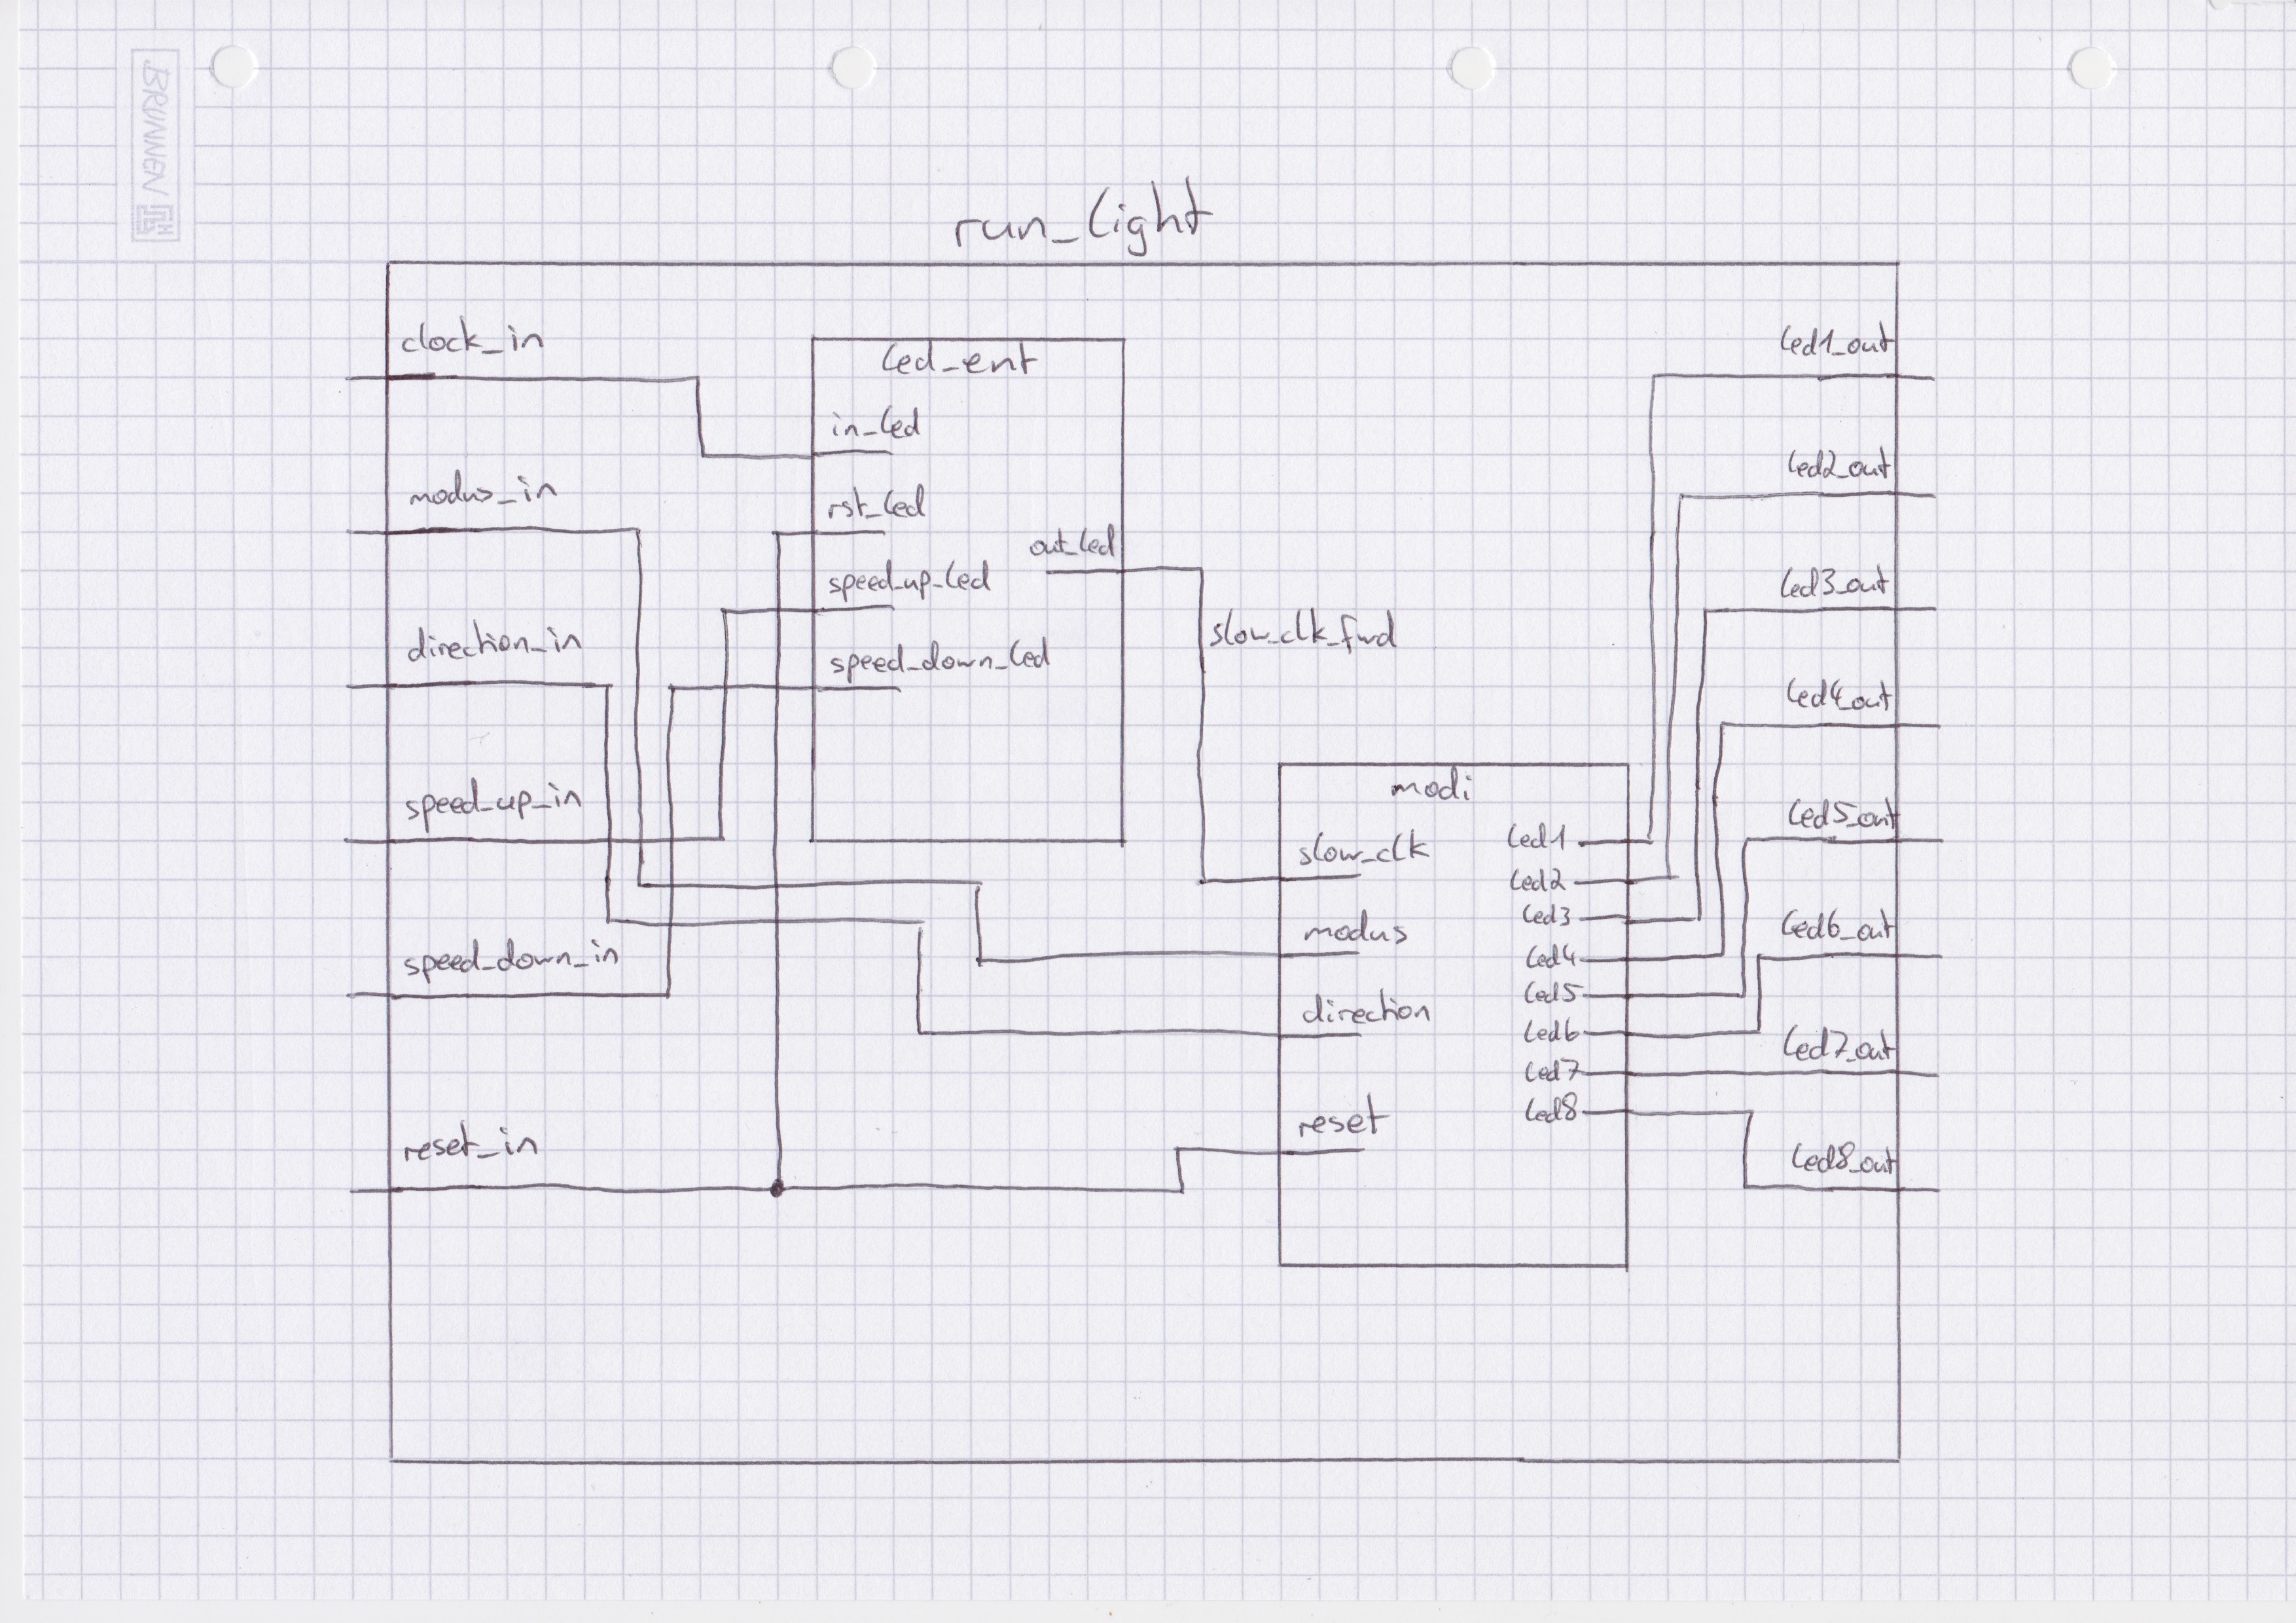
\includegraphics[scale=0.1]{Bilder/runlight.jpeg} \newline
			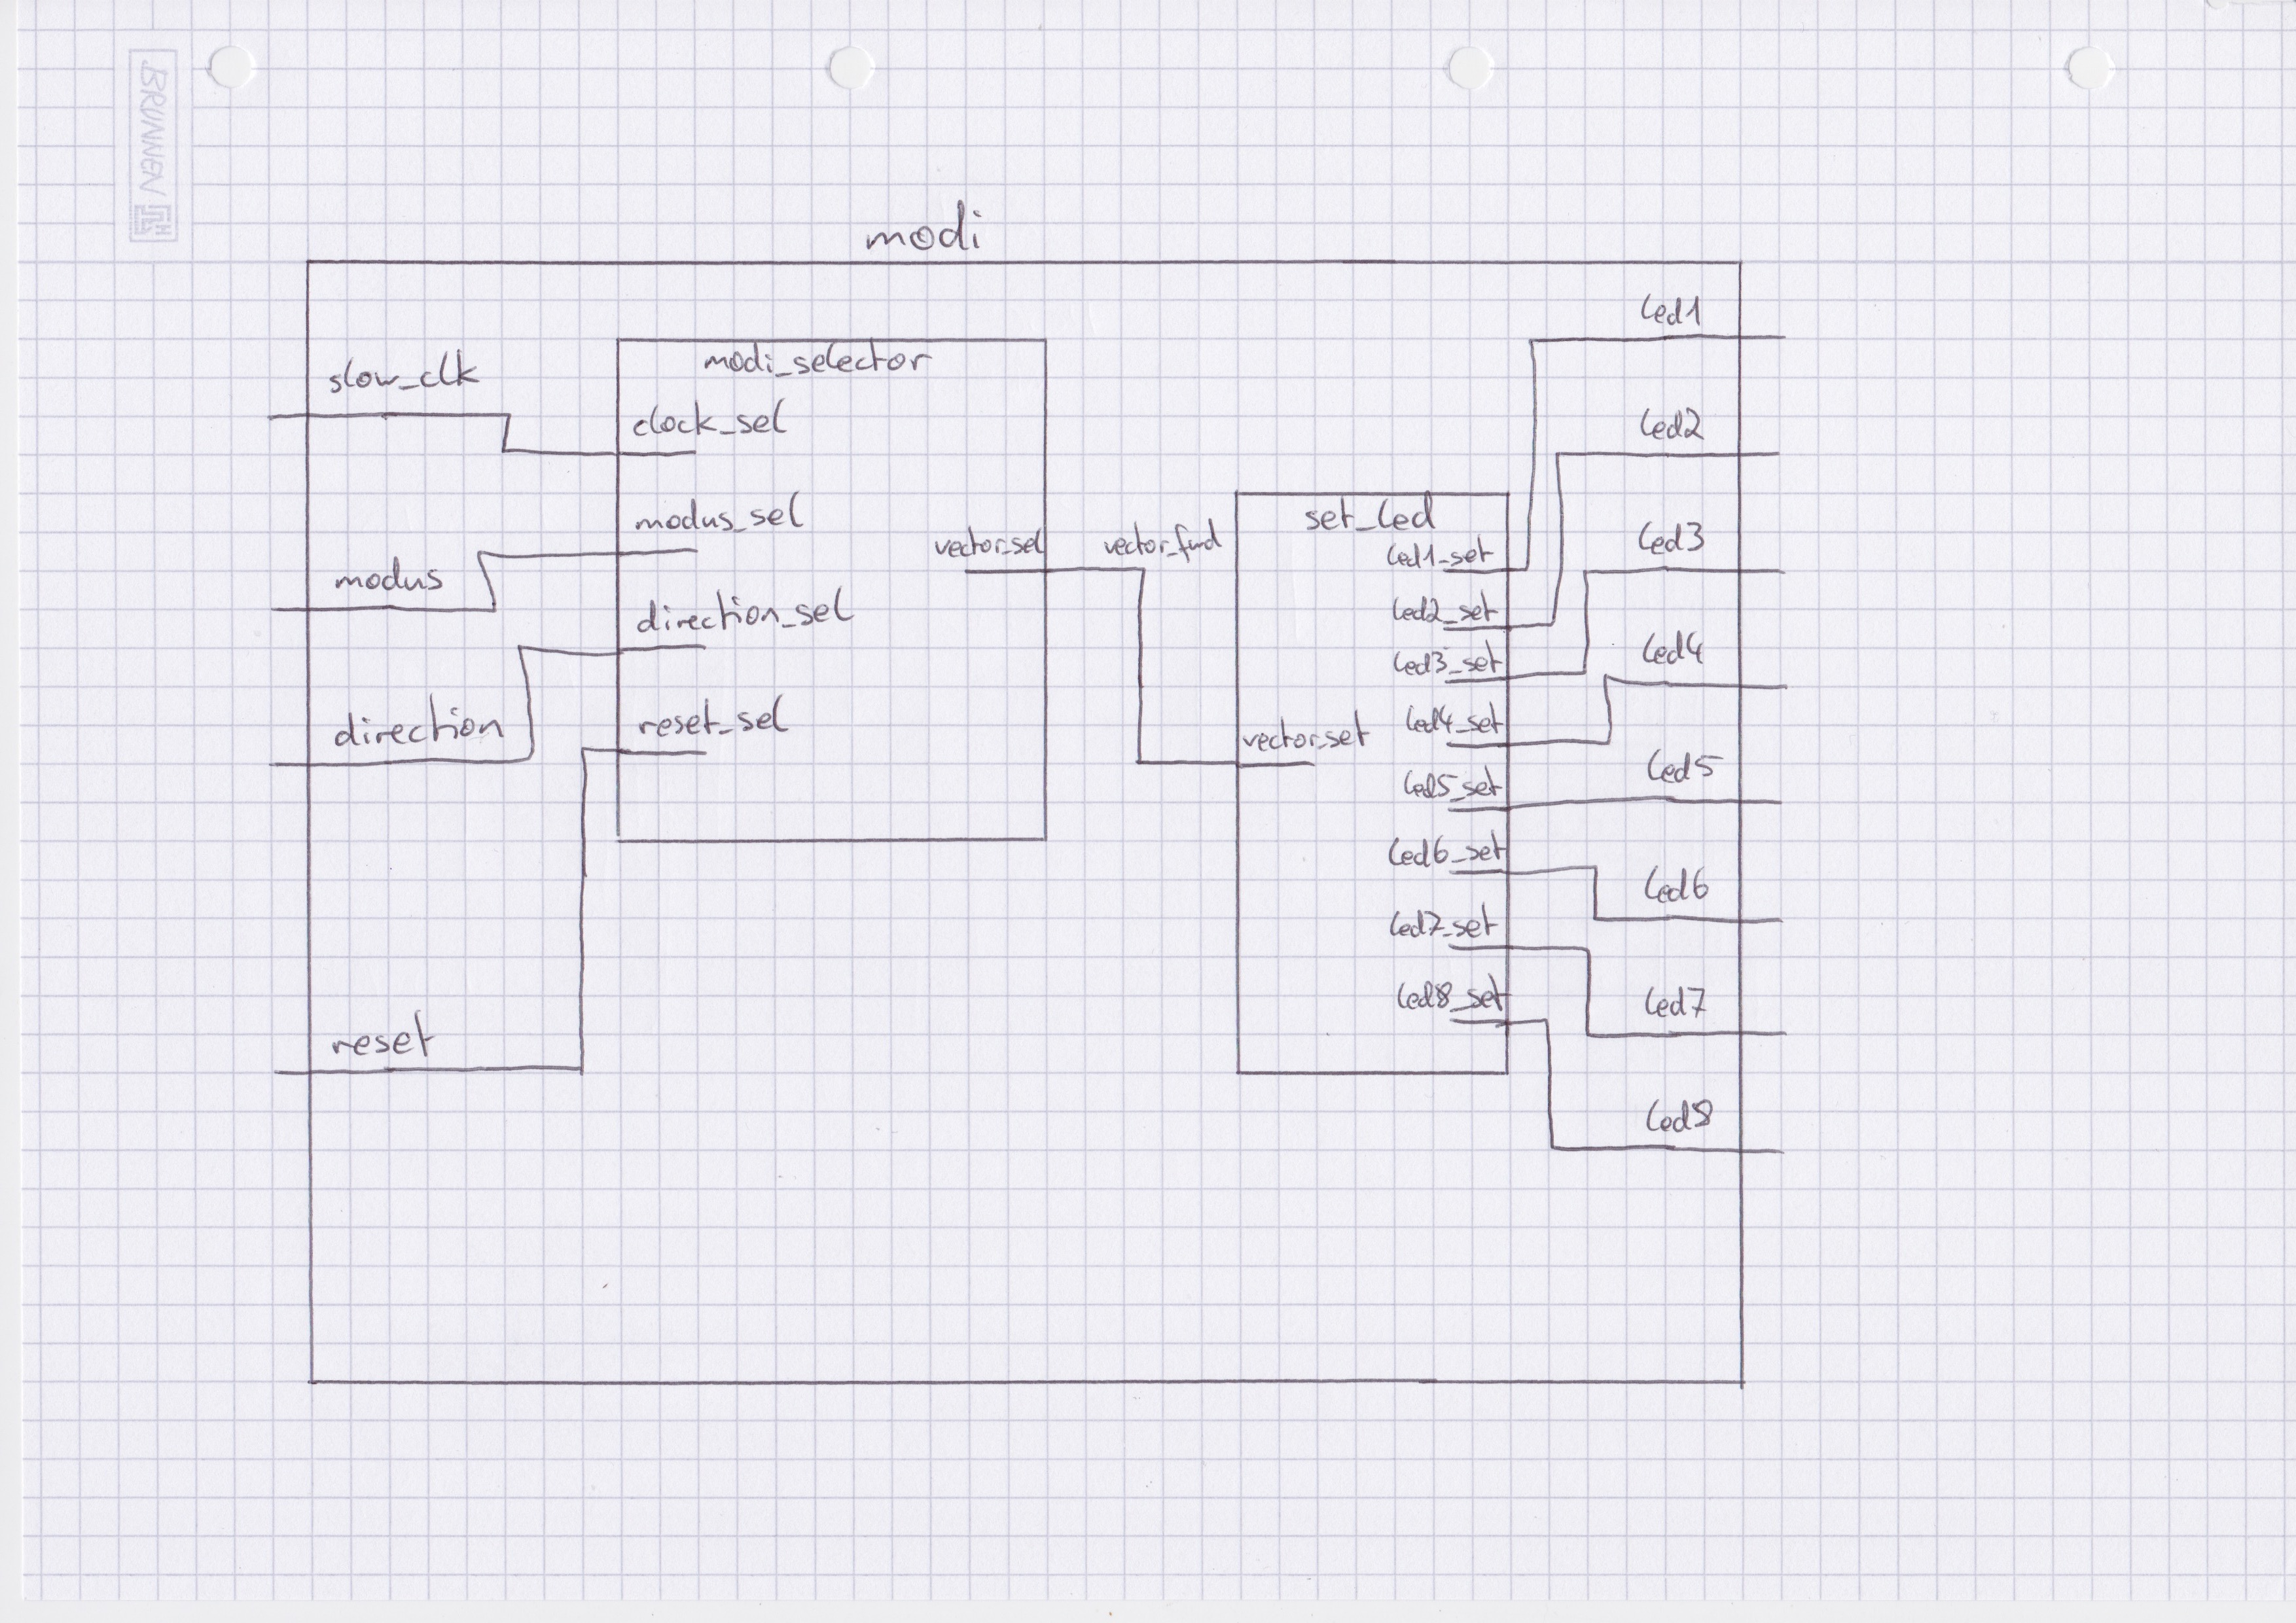
\includegraphics[scale=0.1]{Bilder/modi.jpeg} \newpage
			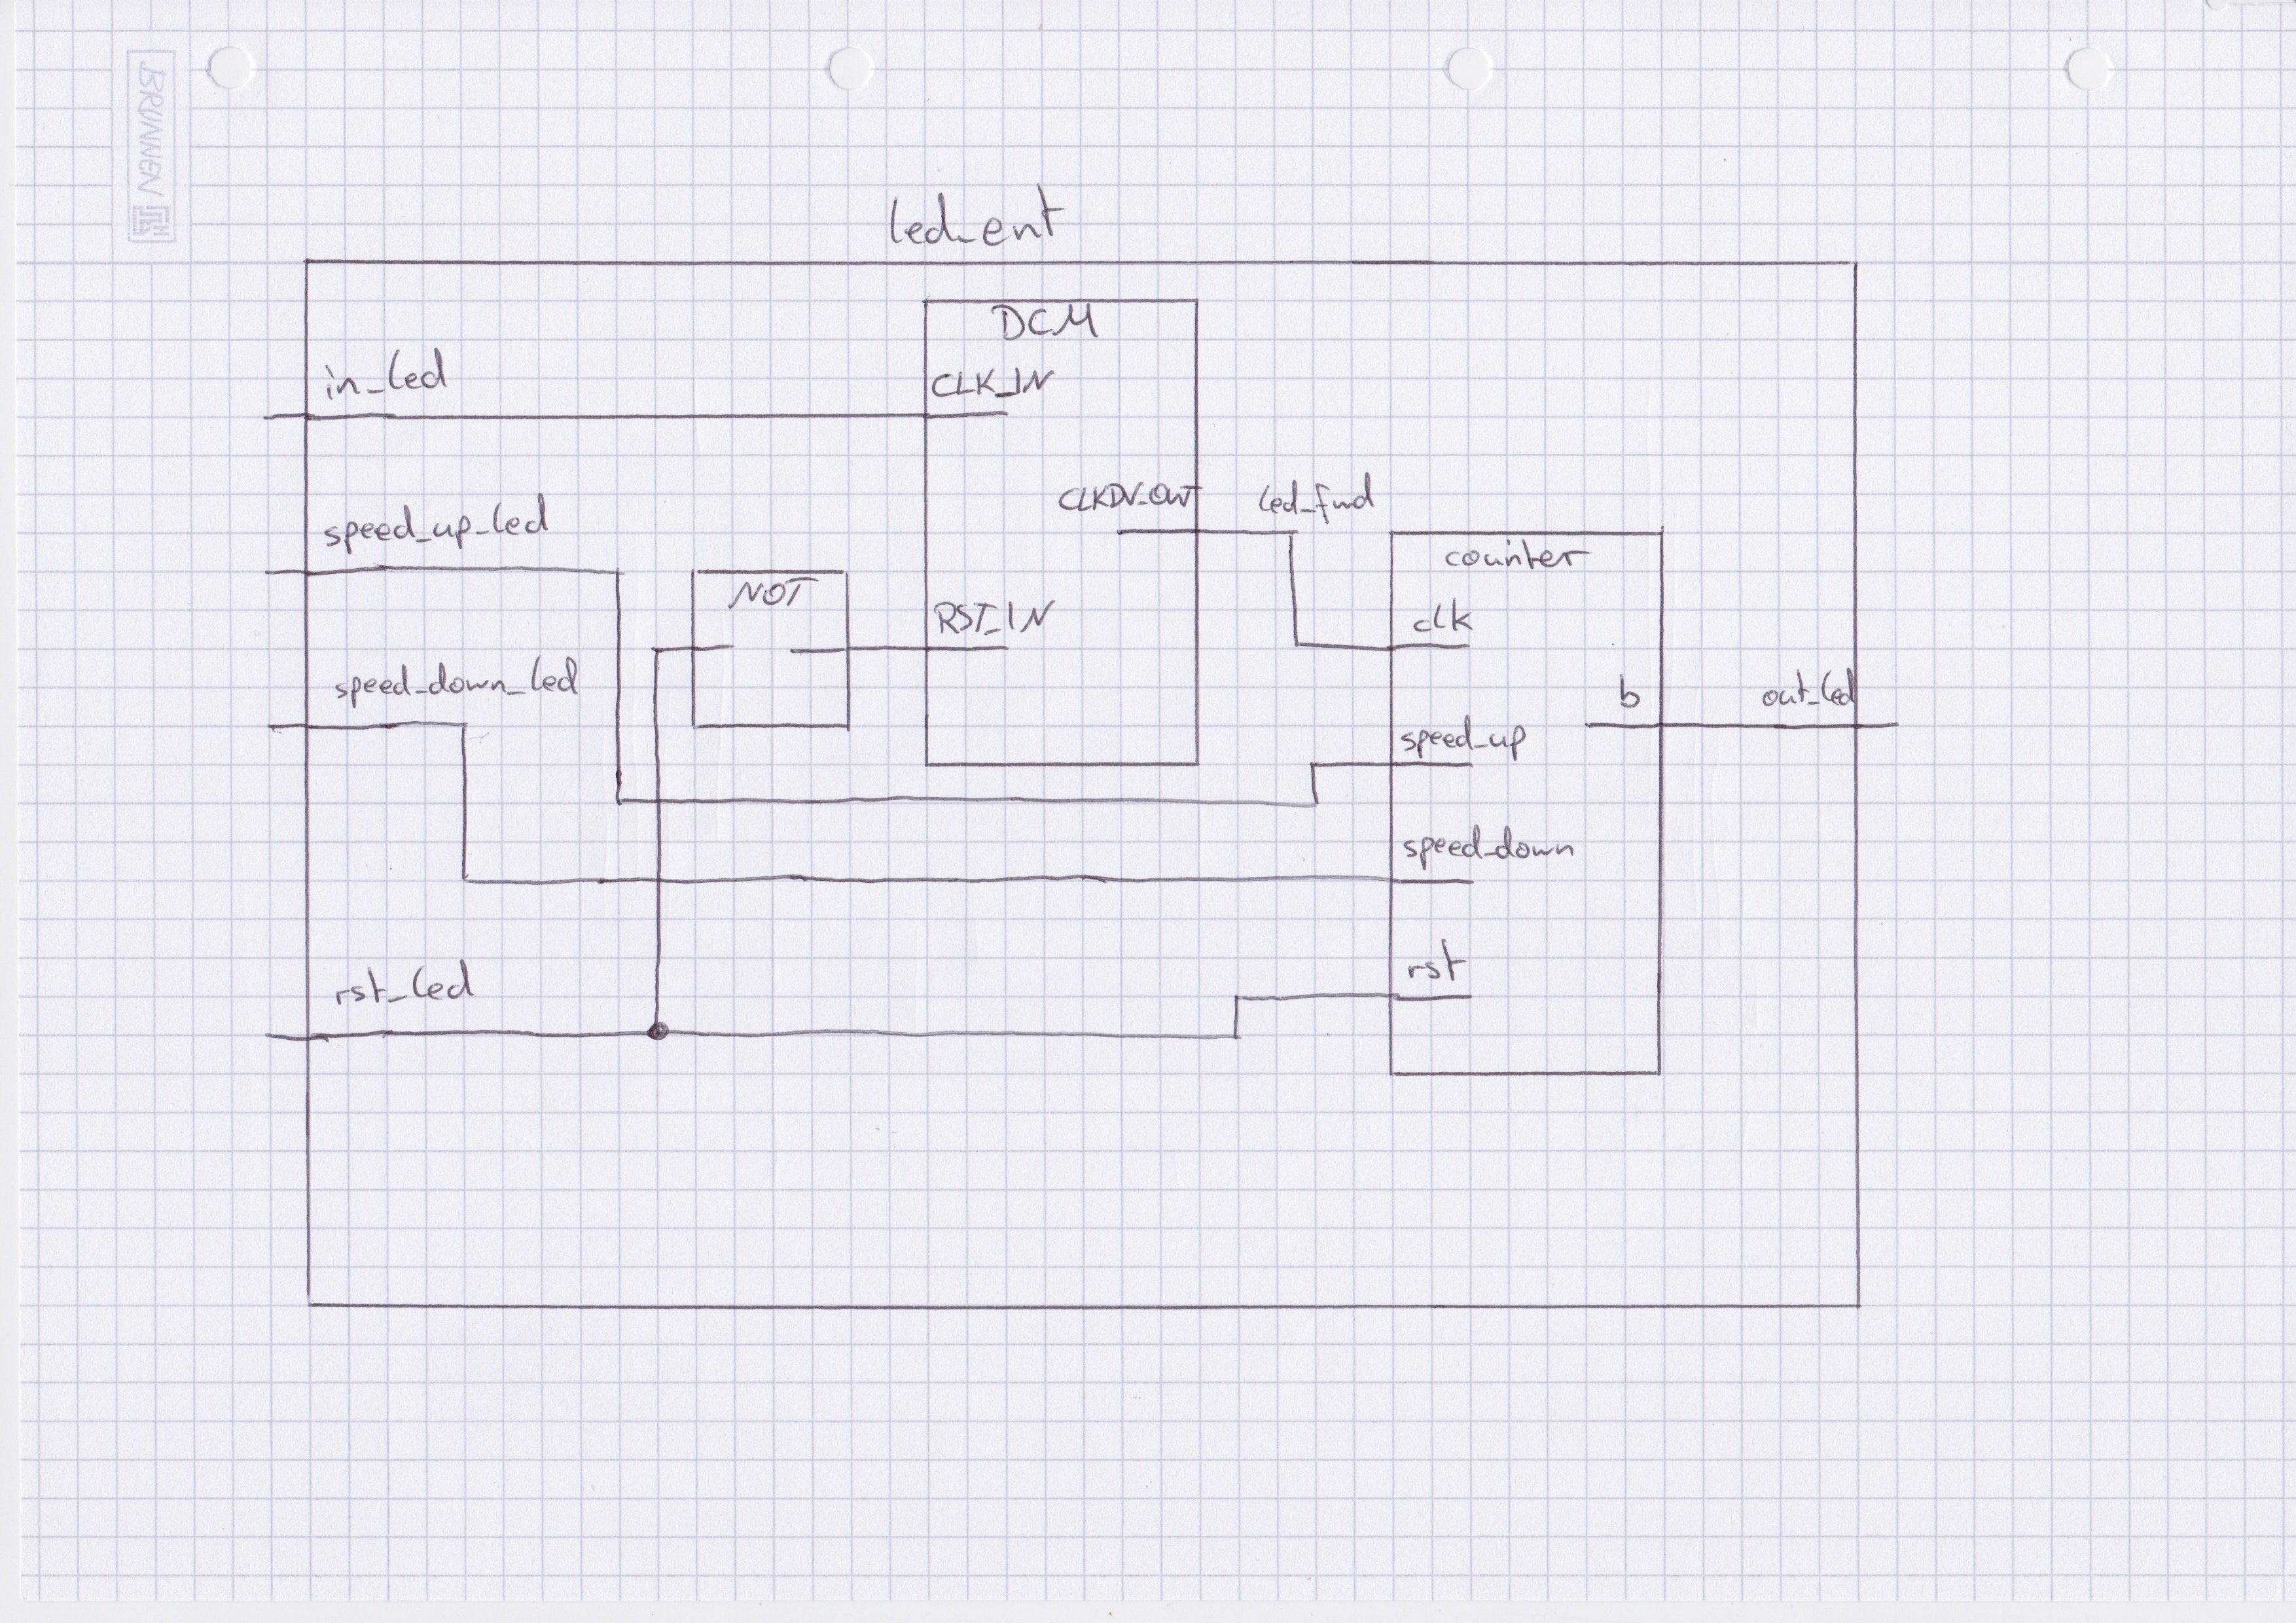
\includegraphics[scale=0.1]{Bilder/ledent.jpeg}
	\section*{Aufgabe 7: Bitmuster}
		Nachdem wir bei dieser Aufgabe auf einen Ansatz für die Lösung kamen, gab es keine Probleme bei der Implementierung.
	
	
\end{document}\grid
\grid
